\documentclass[11pt,letterpaper]{article}
\usepackage[utf8]{inputenc}
\usepackage{graphicx}
\usepackage{linguex}
\usepackage{natbib}%[authoryear,round]{natbib}

\title{Supporting Information}

\author{Jonathan Phillips \& Fiery Cushman}
\date{}

\begin{document}

\maketitle

\section*{SI Text}

\subsection*{Event Ratings} Participants were randomly assigned to rate either the probability, rationality, or morality of each of the 144 events. Those who rated the probability of each action answered the question `How likely is [Agent] to [event]' on a scale from 1 (`Very likely') to 5 (`Very unlikely'); Those who rated the rationality of each action answered the question `How irrational would it be for [Agent] to [event]' on a scale from 1 (`Totally rational') to 5 (`Totally irrational'). Those who rated the morality of each action answered the question `How morally wrong would it be for [Agent] to [event]' on a scale from 1 (`Totally morally fine') to 5 (`Totally morally wrong'). In all cases, participants had an option to respond that the question was `Not applicable'. Participants saw all six of the contexts in random order, and after reading each context, provided a rating of each of the 24 events for that scenario (8 ordinary, 4 immoral, 4 improbable, 4 irrational, and 4 impossible) in random order.

All trials on which participants provided `NA' responses were excluded, and the remaining responses were analyzed to ensure that the a priori categorization of the events was confirmed (see Figure S\ref{eventRatings}). These ratings confirmed our categorization. As a group, `ordinary' events were judged to be less unlikely than improbable events, $t(44)=-13.789$, $p<.001$, $d=4.07$, less irrational than irrational events, $t(38)=-16.536$, $p<.001$, $d=5.23$, and less morally wrong than immoral events, $t(34)=-20.375$, $p<.001$, $d=6.79$. Improbable events, in addition to being perceived as more unlikely than ordinary events, were also less irrational than irrational events, $t(38)=-6.810$, $p<.001$, $d=2.15$, and less morally wrong than immoral events, $t(34)=-17.893$, $p<.001$, $d=5.99$. Unsurprisingly, impossible events were judged to be more improbable than any other group of events, including improbable events, $t(44)=3.888$, $p<.001$, $d=1.15$, and more irrational than any other group of events, including irrational events, $t(26.27)=5.163$, $p<.001$, $d=1.63$. They were not judged to be particularly immoral, and much less immoral than immoral events, $t(34)=-10.143$, $p<.001$, $d=3.38$. Immoral events, in addition to being more immoral than all other events, were judged to be relatively unlikely and irrational. Critically however, they were not judged to be any more unlikely than improbable events, $t(44)=0.028$, $p=.978$, $d<0.01$, and were judged to be marginally less irrational than irrational events, $t(38)=-1.865$, $p=.070$, $d<0.59$. Similarly, irrational events, though unsurprisingly rated as unlikely, were not judged to be more unlikely than improbable events, $t(44)=1.637$, $p=.110$, $d<0.483$. They were, however, rated as less morally wrong than immoral events, $t(38)=-10.488$, $p<.001$, $d<3.50$. Accordingly, the patterns observed for the immoral and irrational events, but not for the improbable or impossible events, must be explained by their elevated levels of immorality and irrationality, rather than the extent to which these events violated descriptive norms.

\begin{figure}
    \centering
    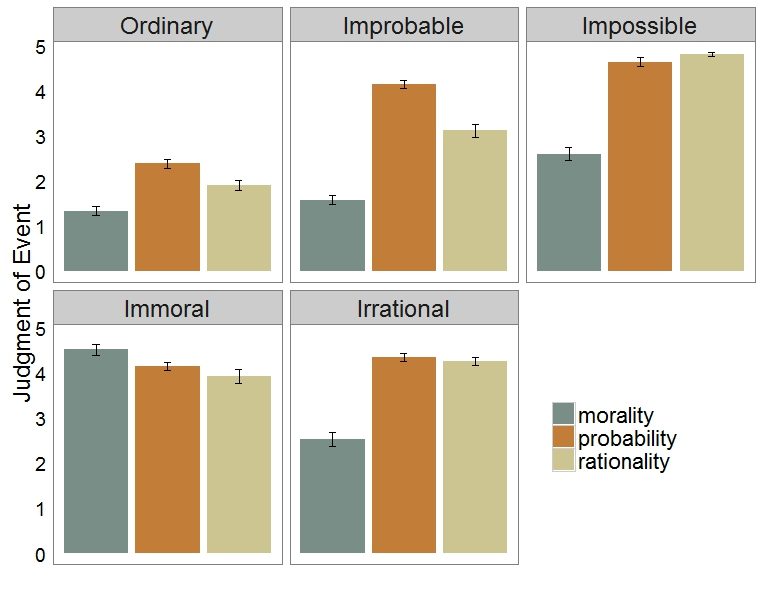
\includegraphics[width=.9\linewidth]{eventRatings}
    \caption{Participants' ratings of the probability, rationality, and morality of the 144 events, split by a priori event category. Error bars depict +/- 1 SEM}
    \label{eventRatings}
\end{figure}


\subsection*{Statistical approach} When possible, the primary analyses were conducted with generalized linear mixed effects models \citep{jaeger2008categorical} in \textsf{R} \citep{bates2014lme4}. The significance of each effect was determined by comparing a model that included the relevant term in the model (as well as other factors that were not currently being investigated) to a model that did not include that term (but did include the other factors not under investigation). The effect was determined to be significant if the fit of the model including the relevant term differed significantly from the fit of the model that did not include that term \citep{barr2013random}.

\subsection*{Differences across modal auxiliaries}

It is widely known that some modal terms demonstrate a preference for more `metaphysical' readings (e.g., `possible', `could') and thus primarily concern the possible ways things could occur. Other modal terms demonstrate a preference for a `circumstantial' reading (e.g., `might', `may'), and thus concern the way that things would normally proceed in the circumstances. Others instead demonstrate a preference for `deontic' readings (e.g., `ought', `should'), and concern what would be morally good or rationally appropriate. The differences between these different modal terms was reflected in participants' judgments. Collapsing across speeded and reflective responses, judgments of what was `possible' and what `could' occur were most concerned with descriptive norms but not prescriptive norms ($t$'s $> 3.62$, $p$'s $< .001$, $d$'s $>0.738$). Judgments of `might' and `may' were roughly equally sensitive to both prescriptive and descriptive norms ($t$'s $< 1.95$, $p$'s $> .05$, $d$'s $<0.397$). And judgments of `should' and `ought' were specifically sensitive to prescriptive norm violations but less sensitive to descriptive norm violations ($t$'s $< -3.15$, $p$'s $< .003$, $d$'s $>0.644$), as would be expected (see Fig. \ref{fig2}).

\begin{figure}
    \centering
    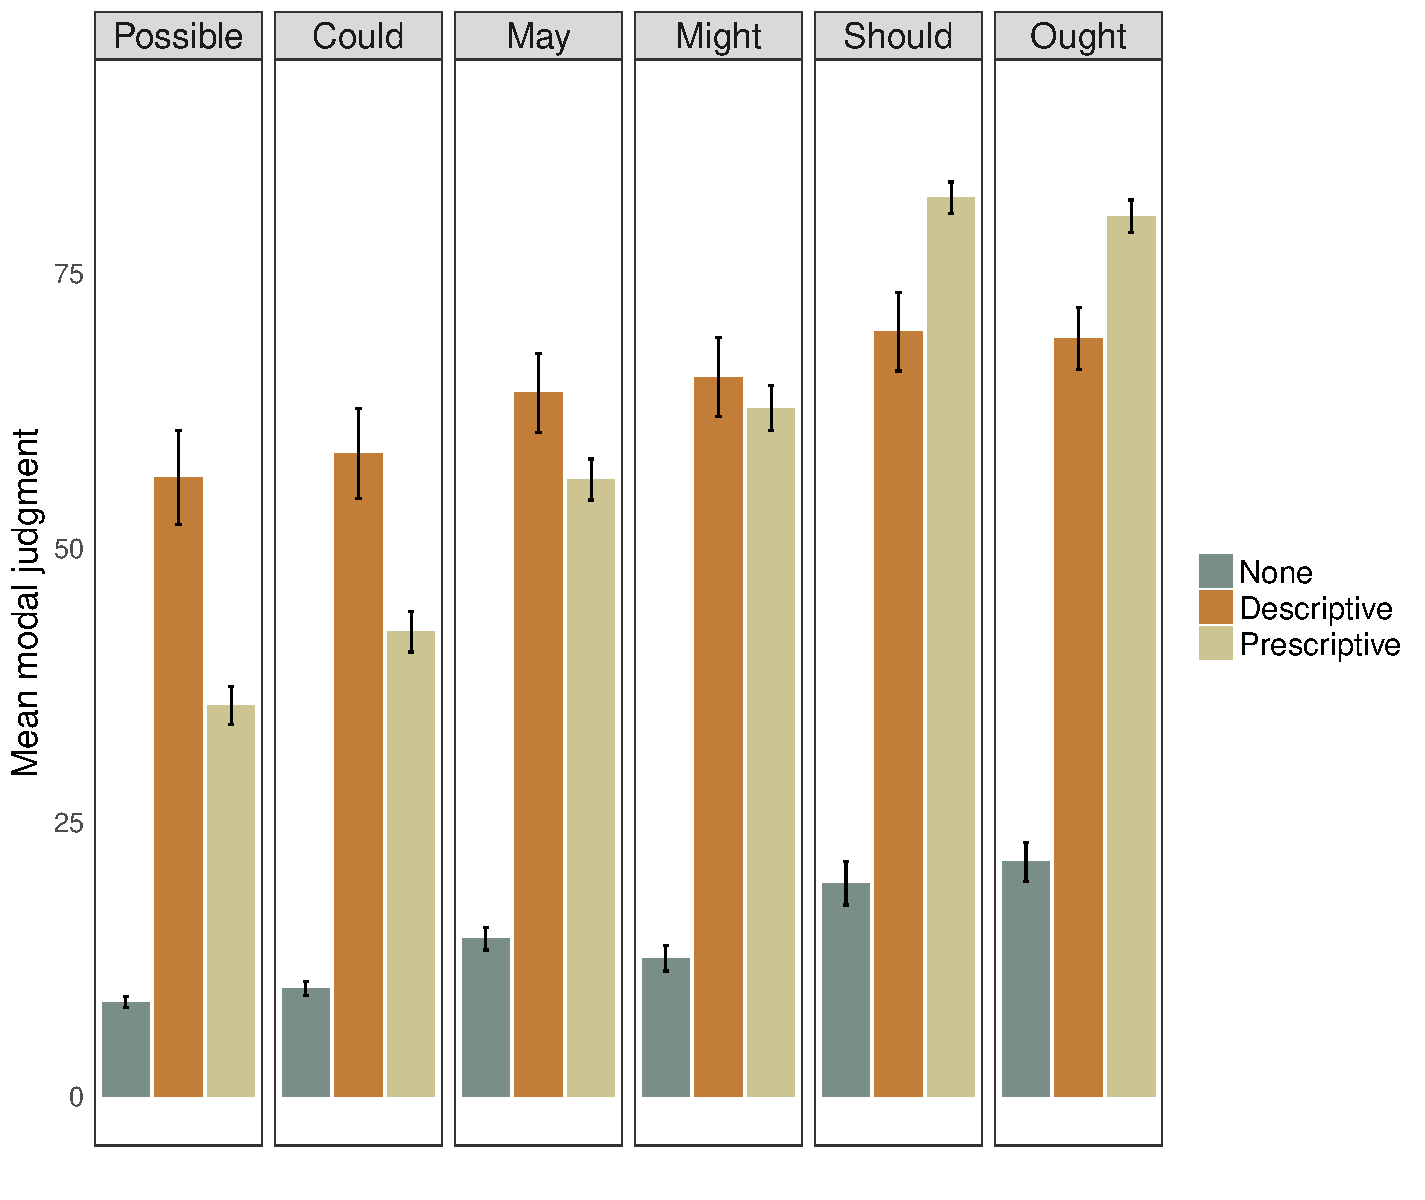
\includegraphics[width=.9\linewidth]{fig2a}
    \caption{Mean judgments for the six different modal terms for events where there were no salient norm violations (in grey), events where only descriptive norm violations were salient (in orange) and events where prescriptive norm violations were relevant (in tan). Error bars depict +/- 1 SEM}
    \label{fig2}
\end{figure}

\subsubsection*{Within-modal correlations}

Given these differences in the modal terms, a natural corollary of our findings in Study 2 is that for events involving prescriptive norm violations, deontic modal judgments made under time pressure and after deliberation should be highly correlated, because moral norms will influence participants' judgments either way. Thus for example, reflective judgments of whether an immoral or irrational action `ought' to be done should be highly correlated with speeded judgments of whether that action `ought' to be done. By contrast, speeded and reflective judgments  of circumstantial modals such as `might' should be less correlated, and more metaphysical modals such as `possible' should be even less correlated. Consistent with this prediction, we found that the similarity of speeded and reflective judgments of deontic modals were highly correlated ($r_{ought} = 0.537$; $r_{should} = 0.531$), that circumstantial modal judgments were relatively less correlated ($r_{may} = 0.407$; $r_{might} = 0.390$), and that metaphysical modal judgments were even less correlated ($r_{could} = 0.358$; $r_{possible} = 0.376$).


\subsection*{Study 3b: Can inferences about agents' desires explain the impact of norms on judgments of `force'?}

The results of Study 3a provide evidence that the impact of norms on deliberative judgments of `force' are best explained by implicit, default representations of possibility. This account relies on the relatively standard assumption that alternative possibilities play a central role in judgments of `force'; see, e.g., \cite{aquinas1952summa,rowe2002nicomachean}; see \cite{mandlekern2017force} for a formal exposition of the semantics of `force' along these lines. 

An alternative possibility, however, is that prescriptive and descriptive norms instead influenced judgments of force by changing participants' inferences about the agent's desires (and thus the default representation of possibilities did not play a direct role). According to this explanation, when an immoral or statistically unlikely event was proposed to the agent, participants were likely to infer that the agent had a strong desire to not do that action, which in turn led them to see the agent as forced to do some other action instead.\footnote{We'd like to thank an anonymous reviewer for raising this alternative way of accounting for the impact of norms on judgments of force.} If correct, this alternative explanation would undermine the earlier evidence that the default representations of possibility play a role in high-level deliberative judgments of force. 

To test this alternative proposal, we collected data on participants' inferences about the agents' desires to not do the proposed action. Similar to Study 3a, participants first read the six different background contexts used in the previous studies, and then read a continuation of that context in which another person proposes that the agent pursue one of the ordinary, immoral, irrational, or improbable event. Participants were then told that the agent always decided to pursue some specified alternative course of action, regardless of the advice given. After reading each background context, participants rated their agreement on a scale from a 1 (`completely agree') to 5 (`completely disagree') with a statement that the agent did not want to do the alternative proposed action. For example, in the scenario in which Josh's father suggests that he could sneak onto public transportation, but Josh ignores his suggestion and books the next available flight, participants were asked whether they agreed or disagreed with the following statement:

\ex.[] \label{desire} Josh did not want to sneak onto public transportation.

According to this alternative explanation, participants should perceive the agent as not wanting to do the actions that involved violations of prescriptive or descriptive norms, and moreover, that this difference in inferred desire should explain the pattern of force judgments from Study 3a. We investigated whether this was the case by computing the average desire ratings for each of the proposed events and then asking how these averages related to (i) the different categories of events and (ii) previous judgments that the agent was forced to do the alternative. First, we found that participants' judgments that the agent did not want to do the action were significantly influenced by the kind of action that was proposed, $F(3,116) = 33.73$, $p < .001$, $\eta^2 = 0.466$. Specifically, participants tended to judge that the agent wanted to do proposed actions less when they were immoral ($M = 1.34$, $SD = 0.17$) or irrational ($M = 1.55$, $SD = 0.26$) than when the they were ordinary ($M = 1.89$, $SD = 0.47$), $t$'s $< -3.88$, $p$'s $< .001$, $d$'s $>0.81$. However, we also found that participants judged that the agent \textit{did} want to do the improbable actions ($M = 2.48$, $SD = 0.59$). Presumably, this pattern occurred because these actions had highly good outcomes but were out of the agent's control, e.g., fixing a car by banging on it. 

More importantly, we next asked if these judgments of the agents' desires were a better predictor of judgments of force than the implicit, default representation of possibility. To do this, we first built a linear mixed effects model that included the default representation of the possibility of each event, and then asked whether this model was improved by adding in participants' judgments of whether the agent desired to not do the proposed action. This was not the case, $\chi^2(1) = 0.760$, $p = 0.383$, suggesting that inferences of the agent's desire added little predictive value above and beyond that already accounted for by implicit representations of possibility. Conversely, however, implicit representations of possibility did improve a model that only included judgments of what the agent desired to not do,  $\chi^2(1) = 52.92$, $p < 0.001$. 

Finally, we focused specifically on immoral and irrational events and whether the perceptions of the agents' desires mediated the impact of morality on judgments of force. We found that they did \textit{not} significantly mediate the impact of either immorality (95\%CI [-0.154,0.081], $p = 0.57$), or rationality (95\%CI [-0.098,0.058], $p = 0.53$). These additional analyses further demonstrate the critical importance of implicit representations of possibility in deliberative judgments of force.

\subsection*{Exclusion criteria and supplemental analyses} 

\textbf{Experiments 1b and 2a-e}: Trials on which participants did not respond were excluded from the analyses. Subsequently, each participant's average response time (excluding outlier responses defined as $>6000ms$) was computed. All data from a participant were dropped if a participant's \textit{average} response time was lower than 800ms in the speeded condition or lower than 1000ms in the reflective condition ($\approx6\%$ of participants in Experiment 1a and $\approx8\%$ in Experiments 2a-e). Additionally, data from all trials on which a response was given in less than 500ms were dropped ($\approx1\%$ in Experiment 1a and Experiments 2a-e), as were data from \textit{reflective} trials on which the response was given in less than 1500ms ($\approx27\%$ in Experiment 1 and Experiments 2a-e).
\vspace{5mm}

\noindent \textbf{Supplemental analyses:} To ensure that the key differences we observed did not arise from a selection-effect produced by the unequal exclusion of data from the reflective condition, we reanalyzed the data without the separate exclusion criteria for the reflective condition. While relaxing this exclusion criteria obviously reduces the difference between two conditions, we still continued to observe the key results. In Experiment 1a, we again observed an effect of whether participants were asked to reflectively deliberate, $\chi^2(1) = 18.403$, $p < .001$, an effect of event-type  $\chi^2(4) = 880.23$, $p < .001$, and critically, a deliberation $*$ event-type interaction, $\chi^2(4) = 76.02$, $p < .001$. This interaction effect continued to be driven in party by the fact that participants more tended to judge immoral events were impossible when they responded quickly ($M = 37.30$, $SD = 30.21$), than when they responded after deliberating ($M = 23.23$, $SD = 31.10$), ($z = 4.942$, $p < .001$). Similarly, they  tended to judge that irrational events were impossible more when answering quickly ($M = 42.10$, $SD = 25.89$) than after reflecting ($M = 37.33$, $SD = 28.54$), ($z = 2.115$, $p < .05$)

Moreover, in Experiment 2, we continued to find that modal judgments were significantly more correlated when participants did not have time to reflect ($M_{r} = 0.892$, $SD_{r} = 0.059$) than when they did ($M_{r} = 0.858$, $SD_{r} = 0.106$), $t(14) = 2.341$, $p  = .035$, $d = 0.403$. We additionally continued to observe an interaction effect between the type of norms that were relevant and whether or not participants had time to reflect, $\chi^2(1) = 8.545$, $p = .003$. Decomposing this interaction, we found that for descriptive-norm events, there was no decrease in the correlation between the modal judgments when participants reflected before answering ($M_{r} = 0.912$, $SD_{r} = 0.052$) from when they answered before reflecting ($M_{r} = 0.908$, $SD_{r} = 0.042$), $t(14) = 0.491$, $p  = .631$, $d = 0.077$. Next, we focused on judgments made when prescriptive norms were relevant and found a much larger decrease in the correlations between the modal judgments made when participants reflected before answering ($M_{r} = 0.438$, $SD_{r} = 0.290$), as compared to when they answered before reflecting ($M_{r} = 0.628$, $SD_{r} = 0.145$), $t(14) = 3.569$, $p  = .003$, $d = 0.831$.

Finally, in Experiment 3, we continued to find that deliberative judgments of force were better predicted by speeded judgments of possibility. Specifically, including reflective judgments of possibility did not significantly improve a model that already included non-reflective judgments of possibility, $\chi^2(1) = 0.097$, $p = .756$. In contrast, including non-reflective judgments of possibility did significantly improve a model that already included reflective judgments of possibility $\chi^2(1) = 20.583$, $p < .001$.

\vspace{5mm}
\noindent \textbf{Experiments 1a and 3a-b}: No data were excluded from these experiments as there was no time manipulation.

\clearpage

\bibliographystyle{apalike}
\bibliography{modalSampling}   


\end{document}